\documentclass[review]{elsarticle}

\usepackage{lineno,hyperref}
\usepackage{graphics}
%\usepackage[square,comma,sectionbib,sort&compress]{natbib}  
%\setcitestyle{numbers}
\usepackage{amsmath, amssymb}
\usepackage{dsfont}
\usepackage{fullpage}
\usepackage{bm}
\usepackage{setspace}
\usepackage{bbding}
\usepackage{tikz}
\usepackage{pgfplots}
\usepackage{pgf}
\usepackage{color}
\usepackage{multirow}
\newcommand{\bma}[1]{\mbox{\boldmath $#1$}}
\newcommand{\bu}{ {\bma{u}} }
\newcommand{\bv}{ {\bma{v}} }
\newcommand{\bw}{ {\bma{w}} }
\newcommand{\bD}{ {\bma{D}} }
\newcommand{\bU}{ {\bma{U}} }
\newcommand{\bW}{ {\bma{W}} }
\newcommand{\bX}{ {\bma{X}} }
\newcommand{\bY}{ {\bma{Y}} }

\bibliographystyle{elsarticle-num}
%%%%%%%%%%%%%%%%%%%%%%%%%%%%%%%%%%%%%%%%%%%%%%
%%%%%%%%%%%%%%%%%%%%%%%%%%%%%%%%%%%%%%%%%%%%%%
%%%%%%%%%%%%%%%%%%%%%%%%%%%%%%%%%%%%%%%%%%%%%%

\begin{document}
\begin{frontmatter}

\title{\large \bf Intra-Subject Locally Adjusted Images for Partial Volume Adjustment}  

\author[biostatAddress,cbicaAddress]{Kristin A. Linn\corref{mycorrespondingauthor}}
\cortext[mycorrespondingauthor]{Corresponding author}
\ead{klinn@pennmedicine.upenn.edu}
\author[psychAddress]{Azeez Adebimpe}
\author[psychAddress]{Tinashe M. Tapera}
\author[biostatAddress]{Jenny Shen}
\author[biostatAddress]{Virgil Gonzenbach}
\author[vandyAddress]{Simon N. Vandekar}
\author[biostatAddress]{Alessandra M. Valcarcel}
\author[psychAddress]{Rastko Ciric}
\author[psychAddress]{Adon FG Rosen}
\author[psychAddress]{Phil Cook}
%\author[biostatAddress]{Abdhi Sarkar}
\author[psychAddress]{Kosha Ruparel}
\author[psychAddress]{David R. Rolf}
\author[arminAddress]{Armin Raznahan}
\author[psychAddress]{Ruben C. Gur}
\author[psychAddress]{Raquel E. Gur}
\author[psychAddress]{John A. Detre}
\author[psychAddress,cbicaAddress]{Theodore D. Satterthwaite}
\author[biostatAddress,cbicaAddress]{Russell T. Shinohara}

\address[biostatAddress]{Penn Statistics in Imaging and Visualization Center, Department of Biostatistics, Epidemiology, and Informatics, University of Pennsylvania, Philadelphia, PA, USA}
\address[cbicaAddress]{Center for Biomedical Imaging Computing and Analytics, University of Pennsylvania, Philadelphia, PA, USA}
\address[psychAddress]{Department of Psychiatry, Perelman School of
  Medicine, University of Pennsylvania, Philadelphia, PA, USA}
\address[vandyAddress]{Department of Biostatistics, Vanderbilt University, Nashville, TN, USA}
\address[arminAddress]{Developmental Neurogenomics Unit, National Institute of Mental Health, Bethesda, MD 20814}

\begin{abstract}
Local cortical coupling has been used to study developmental effects related to spatially varying associations between cortical thickness and sulcal depth throughout the brain. In this work, we define Inter-Modal Coupling (IMCo) as subject-specific local coupling between two volumetric images and then leverage IMCo as a general tool to address partial volume (PV) effects in any functional image type measured in volumetric space. We call the proposed IMCo-adjusted functional images Intra-Subject Locally Adjusted (ISLA) images. Using data from the Philadelphia Neurodevelopmental Cohort, we demonstrate that ISLA cerebral blood flow (CBF) images mitigate partial voluming in gray matter. In group-level analyses, we show that using ISLA CBF images increases detection of nonlinear developmental effects compared to using CBF images corrected for PV effects according to an existing method. 
\end{abstract}

\begin{keyword}
Multi-modal imaging, partial volume effects, gray matter density, cerebral blood flow, inter-modal coupling. 
\end{keyword}

\end{frontmatter}

\linenumbers

\section{Introduction}
\label{sec:Intro}
Due to the limited spatial resolution of standard noninvasive brain imaging techniques, many voxels consist of a mixture of gray matter, white matter, and cerebral spinal fluid. The heterogeneity of tissue types within individual voxels contributes to partial volume (PV) effects in a number of imaging types including positron emission tomography (PET), arterial spin labeling (ASL), and measurements derived from these sequences (CITES). Correcting for PV effects is particularly important in studies of adolescent neurodevelopment, since adolescence is a time of rapid changes in the structure and function of the brain. In order to obtain an accurate understanding of changes in function and joint structure-functional relationships throughout development, researchers need to ensure results are not contaminated or driven by PV effects.   

Local covariance patterns between cortical thickness and sulcal depth were studied by \citep{Van+etal:16} using subject-level coupling maps. At each surface-level vertex, coupling was defined as the slope of a weighted least squares regression, where surrounding vertices were weighted by their distance to the center vertex. In this work, we leverage subject-level coupling between function and structure in volumetric space to correct functional image modalities for partial volume (PV) effects prior to group-level analyses. This version of coupling in volumetric space was developed and applied to improve detection of white matter lesions in multiple sclerosis and is referred to as Inter-Model Coupling (IMCo) in that literature \citep{valcarcel2018mimosa,valcarcel2018dual}. For simplicity, we focus on demonstrating the performance of our PV correction using cerebral blood flow (CBF) images. However, our method is applicable more generally to any volumetric functional imaging type (e.g., ALFF, REHO) that may exhibit partial voluming, as long as a structural T1 image is available for all study participants. Broadly, our method for PV correction estimates the parameters of the IMCo model separately for each subject and each voxel using a gray matter density image and a co-registered functional image for which PV correction is desired. We then use the fitted IMCo models to predict what the voxel values of the functional image would be if all voxels contained 100\% gray matter. We refer to the resulting images as Intra-Subject Locally Adjusted (ISLA) images.

A number of established approaches for PV correction apply directly to arterial spin labeling (ASL) image data \citep{asllani2008regression, chappell2011partial}. In \citep{asllani2008regression}, the authors proposed a linear regression-based method applied within local kernels centered at each voxel of a single inversion time (TI), continuous ASL (CASL) sequence. A method for PV correction proposed by \citep{chappell2011partial} leveraged additional information provided by a multi-TI ASL sequence about the local kinetic properties of gray and white matter. Information about the kinetic model parameters is borrowed across voxels by employing a Markov Random Field (MRF) with adaptive spatial priors. This approach is implemented in the BASIL toolset \citep{chappell2008variational} of the FMRIB Software Library \citep{woolrich2009bayesian,smith2004advances,jenkinson2012fsl}.

Our proposed method for PV correction overcomes several limitations of these existing methods. We switch the order of the calculations so that PV correction is performed directly on ASL-derived CBF images. As a result, our method is applicable regardless of the ASL sequence implemented by study investigators. Furthermore, this reordering permits a general PV correction framework that can be applied to any functional imaging type measured in volumetric space. While the approach to PV correction in \citep{ahlgren2014partial} also uses CBF images instead of ASL, it suffers from a poorly specified model with unrealistic assumptions. Furthermore, the model is applied to data from individual slices, ignoring the volumetric nature of CBF and the structural images - white and gray matter density - on which the method depends. ONE MORE SENTENCE DRIVING HOME THAT OUR MODEL IS BETTER.

In Section \ref{sec:Methods}, we briefly describe the PNC imaging sample used to develop our method for partial volume  adjustment and give details about the image processing. In addition, we fully describe the model and estimation procedures used to obtain our proposed PV-corrected images, which we refer to as Intra-Subject Locally Adjusted images (ISLA). In Section
\ref{sec:Results}, we demonstrate the utility of ISLA images as a general way to address partial voluming that is applicable to any volumetric imaging modality when subject-level gray matter density maps are available. We also show evidence using ISLA images in downstream, group-level analyses increases power to detect developmental effects compared to the method developed by \citep{ahlgren2014partial}. We conclude with a discussion in Section \ref{sec:Discussion}. 

\section{Methods}
\label{sec:Methods}

\subsection{Subjects}
\label{subsec:Subjects}

The Philadelphia Neurodevelopmental Cohort is a large study of youths ages 8-21 at enrollment carried out by the University of Pennsylvania (Penn) and the Center for Applied Genomics at the Children's Hospital of Philadelphia (CHOP). Of the 9428 children who underwent thorough cognitive and psychiatric evaluation, 1445 also received multi-modal imaging of the brain at Penn. This sub-sample therefore comprises one of the largest resources for charting normal neurological development in adolescence and learning how deviations from normal neurodevelopmental trajectories correlate with psychiatric conditions, two of the main goals of the study.  The study design and data have been previously described in detail by \citep{Sat+etal:14}. Our final sample consisted of a cross-sectional sample of $n=1132$ subjects who were not currently taking psychoactive medication, did not have any medical problems that could impact brain function, did not have a history of psychiatric hospitalization, did not have any abnormalities of brain structure or distortions of brain anatomy as determined by review of the T1 image by a neuroradiologist, and had sufficient T1 and CBF image quality. 
%From this sample, \textcolor{red}{???} individuals were excluded for insufficient T1 image quality. Modality-specific exclusions based on quality of the functional images are described in the next section. 

\subsection{Image Acquisition and Preprocessing}
\label{subsec:Preprocessing}

All neuroimaging data were acquired on the same Siemens TIM Trio 3 Tesla, 32 channel head coil scanner. Structural image processing used tools included in ANTs \citep{avants2009advanced}. In order to avoid registration bias and maximize sensitivity to detect regional effects that can be impacted by registration error, a custom adolescent template and tissue priors were created using data from 140 PNC participants, balanced for age and sex. Structural images were then processed and registered to this template using the ANTs cortical thickness pipeline \citep{tustison2014large}. This procedure included brain extraction, N4 bias field correction \citep{tustison2010n4itk}, and Atropos tissue segmentation \citep{avants2011open}. Gray matter density was calculated using Atropos, which employs an iterative segmentation procedure that is initialized using 3-class K-means segmentation. This procedure produces both a discrete 3-class hard segmentation as well as a probabilistic gray matter density map for each subject. We used the probabilistic gray matter maps to estimate the parameters in our model for obtaining ISLA images and both the probabilistic gray and white matter maps to perform PV correction using the comparator method of \citep{ahlgren2014partial}.

Perfusion imaging employed a custom pseudocontinuous arterial spin labeling (pCASL) sequence \citep{Wu+etal:07}, with details available in the Supporting Information of \citep{Sat+Shi+etal:14}. \textcolor{red}{For each subject, CBF was estimated from the pCASL sequence by NEED BBL HELP HERE AND CITATION.} 

\subsection{Inter-Modal Coupling (IMCo) of CBF and GMD}
\label{subsec:IMCo}

In \citep{Van+etal:16}, coupling at a specific location on the cortex was defined as the estimated slope from a locally weighted regression of gyral thickness on sulcal depth. This value was computed at the subject level using data from nearby cortical vertices that were weighted based on their distance to the location of interest. In practice, the number of vertices in the neighborhood used to estimate coupling is a tuning parameter that must be specified by the user. Similarly, we defined Inter-Modal Coupling (IMCo) at a particular voxel in the brain as the estimated parameters from a locally weighted regression of CBF on GMD, where both images had been registered to the PNC template space. For all analyses in this paper, IMCo was calculated in a custom PNC template space (see Section \ref{subsec:Preprocessing}). However, we note that IMCo can alternatively be calculated in native space between co-registered images.  

Formally, let $v^{*}$ denote an arbitrary voxel in the brain and $\mathcal{V}$ a neighborhood of surrounding voxels centered at $v^{*}$. Define $d(v, v^{*})$ to be a measure of distance from voxel $v \in \mathcal{V}$ to $v^{*}$, such as Euclidean distance. Let $K$ be the size of the voxel neighborhood, i.e., $K \triangleq |\mathcal{V}|$. Let ${\bf X}_{i}(v^{*})$ denote subject $i$'s vectorized GMD image voxels from neighborhood $\mathcal{V}$ centered at voxel $v^{*}$ and ${\bf Y}_{i}(v^{*})$ the corresponding vectorized CBF image voxels. Using this notation, we assume the following model:

\begin{equation}
\label{mdl1}
{\bf Y}_{i}(v^{*}) = \beta_{0, i}(v^{*}) + {\bf X}_{i}(v^{*})\beta_{1, i}(v^{*}) + \epsilon_{i}(v^{*}),
\end{equation} 

where $E[\epsilon_{i}(v^{*})] = 0_{V \times 1}$ and $Var[\epsilon_{i}(v^{*})] = \Omega_{i}(v^{*})$. Since we can't identify a separate covariance matrix for each subject at each location, we reduce the parameter space by assuming a common covariance structure for all $i$ and $v^{*}$, $Var[\epsilon_{i}(v^{*})] = \Omega$. We fit (\ref{mdl1}) using weighted least squares which is based on the specification of a diagonal $\Omega$. The diagonal elements correspond to voxel-level weights that downweight neighborhood voxels that are further from the center voxel, $v^{*}$.


The following steps broadly describe the IMCo estimation procedure for subject $i$, with specific details given below: 

\begin{enumerate}
\item For each voxel $v \in \mathcal{V}$, assign a weight, $w_{v^{*}}^{d}(v)$, that depends on $d(v, v^{*})$. Define $W = \text{diag}({\bf w}_{v^{*}}^{d})$, where ${\bf w}_{v^{*}}^{d}$ is the $K \times 1$ vector of neighborhood weights and the off diagonal elements are all 0.

\item Use weighted least squares to estimate $\bma{\beta}_{i}(v^{*}) \triangleq (\beta_{0, i}(v^{*})^{T}, \beta_{1, i}(v^{*}))$ in model (\ref{mdl1}). Let $\tilde{\bf X}_{i}$ be a design matrix that includes a column of 1s for the intercept and a column corresponding to ${\bf X}_{i}$. To simplify notation we drop the dependence on $v^{*}$ on the right hand side in the following solution for $\bma{\beta}_{i}(v^{*})$: 

\begin{equation*}
\hat{\bma{\beta}}_{i}(v^{*}) = (\tilde{\bf X}_{i}^{T}W\tilde{\bf X}_{i})^{-1}\tilde{\bf X}_{i}^{T}W{\bf Y}_{i}.
\end{equation*} 

\item Define the estimated intercepts and slopes from the weighted regressions in Step 2 as the set of IMCo estimates for subject $i$, i.e., $\hat{\bma{\theta}}_{i} \triangleq \{ \hat{\bma{\beta}}_{i}(v^{*}) \}_{v^{*} = 1}^{V}$, where $V$ is the total number of voxels in a region of interest (e.g., a template-space gray matter mask).
\end{enumerate}

\noindent We applied this procedure to all subjects and voxels, $v^{*} \in {1, \dots, V}$, within the intersection of a 10\% gray matter mask derived from a custom template (see Section \ref{subsec:Preprocessing}) and a mask of reliable ASL signal coverage. We will refer to this space as the gray matter region of interest (GM-ROI). As a sensitivity analysis, we repeated the analyses using the ASL coverage mask intersected with a 20\% gray matter mask (results provided in the Supplementary Material). When an IMCo neighborhood contained voxels outside of the GM-ROI, those voxels were not included in the locally weighted IMCo regression step. However, as long as the center voxel $v^{*}$ and a minimum of three neigborhood voxels were contained in the GM-ROI, IMCo estimation was performed at $v^{*}$. 

In Step 1 of the IMCo estimation procedure, we used Euclidean distance for $d$, but other distance measures could be specified. In addition, we employed weights from an isotropic Gaussian kernal, 
\begin{equation}
\label{k1}
w_{v^{*}}^{d, \sigma}(v) = e^{-\frac{d(v, v^{*})^2}{2\sigma^2}},
\end{equation}
where the parameter $\sigma$ determines the smoothness of the estimated IMCo measures across the brain. From equation (\ref{k1}), it can be seen that the center voxel $v^{*}$ receives weight $w_{v^{*}}^{d, \sigma}(v^{*})=1$, and the weights of voxels in the regression neighborhood decreas as a function of distance to the center voxel $v^{*}$. 

It can also be seen from equation (\ref{k1}) that larger values of $\sigma$ corresponded to smoother IMCo images. We specified $\sigma$ based on the full width half mass (FWHM) parameter of a univariate Gaussian distribution, with FWHM units measured in millimeters. Although the Gaussian distribution has infinite support, small weights were rounded to zero to obtain a finite neighborhood of positively weighted voxels that reduced the memory requirements of the procedure. In Section \ref{sec:Results}, we used a FWHM of 3 millimeters (mm) which resulted in a 7x7x7 voxel neighborhood of non-zero weights. Since each voxel had a resolution of 2x2x2mm, the neighborhood was 14mm cubed. To assess the sensitivity to neighborhood  size, we repeated the analysis using a larger FWHM of 4mm and a smaller FWHM of 2mm, which resulted in neighborhoods of size 9x9x9 voxels (18mm cubed) and 5x5x5 voxels (10mm cubed), respectively. 

\begin{figure}
\begin{center}
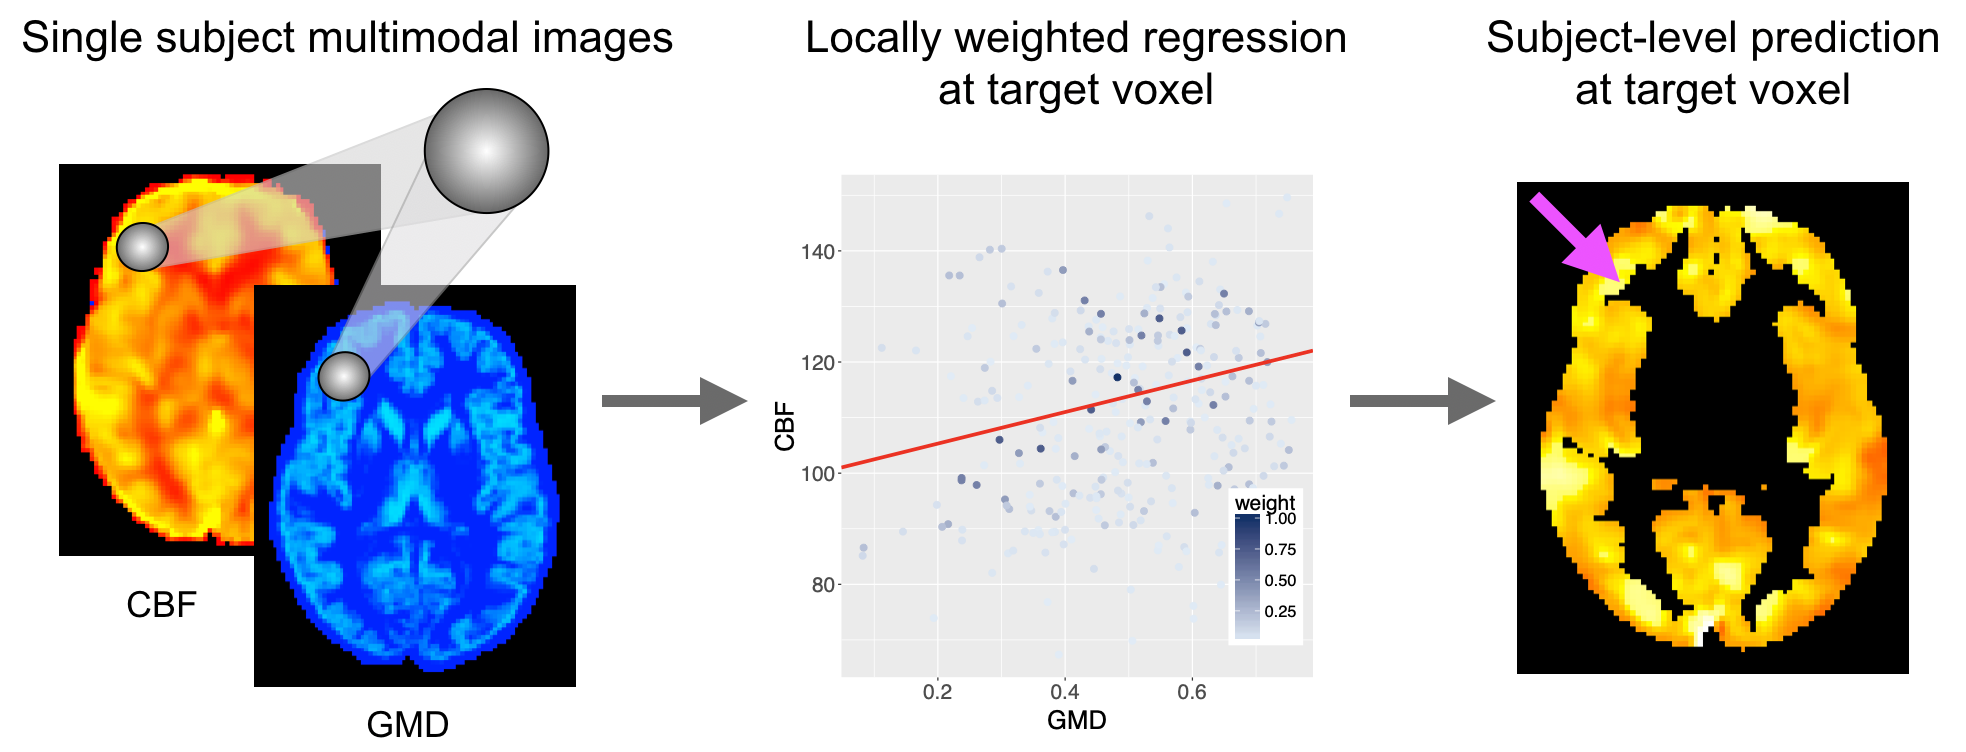
\includegraphics[scale=.5]{figures/schema.png}
\end{center}
\caption{\emph{Illustration of the ISLA estimation procedure for a single individual and target voxel centered within the gray sphere.}}\label{schema} 
\end{figure}

\subsection{Partial Volume Corrected CBF Images}
\label{subsec:ISLA}

The ISLA CBF image for a given individual is defined as the predicted image obtained by setting GMD=1 at each voxel in the GM-ROI; all voxels outside the GM-ROI were set to 0. More specifically, given the IMCo estimates for subject $i$ at voxel $v$, the ISLA CBF value was calculated as $\hat{y}_{i}(v) = \hat{\beta}_{i, 0}(v) + \hat{\beta}_{i, 1}(v)$. This predicted value represents a model-based estimate of what value would have been observed had voxel $v$ been composed of 100\% gray matter, i.e., no partial voluming at its location. Figure \ref{schema} illustrates the ISLA CBF estimation procedure for an individual subject and single target voxel. 

The method proposed by \citep{ahlgren2014partial} is similar to our proposed method in that a model is specified and fit within local neighborhoods centered at each voxel in the GM-ROI. However, there are three key deviations from our approach: 1) an unweighted linear regression is fit in each neighborhood; 2) the design matrix within each neighborhood includes terms for gray matter density and white matter density but no intercept; and 3) the regression models are fit within 2D neighborhoods defined separately in each slice. After estimating all model parameters from this procedure, the coefficient corresponding to the gray matter term is taken as the estimate of partial volume corrected CBF. We note that by not weighting voxels within the local regression neighborhoods, this method is assuming an independent correlation structure throughout the brain, which is unlikely to hold in practice given the strong spatial correlation of imaging data. When comparing ISLA CBF to this method, which we refer to as the unweighted correction (UC), we made one modification which was to use a 3D kernel. We believe this modification facilitates a fair comparison of the methods since the results will be subject to the same amount of smoothing induced by the isotropic kernel.

For each subject in our PNC sample, we computed ISLA CBF and UC CBF. We first assessed the results by visualizing pairwise differences between the average CBF, average ISLA CBF, and average UC CBF images. To determine whether the performace of the PV correction methods differed by GMD, we plotted the distribution of (corrected and uncorrected) average CBF across voxels within 10\% increments of GMD.  

\subsection{Developmental Effects}
\label{subsec:flameo}

Separately for each of the corrected and uncorrected CBF images as outcomes, we performed a voxelwise analysis to identify regions of the brain for which there was evidence of nonlinear age by sex interactions. DESCRIBE MODEL, ESTIMATION, AND SUMMARY STATISTICS OF INTEREST.


\section{Results}
\label{sec:Results}   

\begin{itemize}
\item Figure XX displays the average CBF, average ISLA CBF, and average UC CBF images, as well as all pairwise differences. These will show increased values of ISLA CBF compared to CBF near tissue class boundaries. \textcolor{red}{Should we show this on surface or in volume space? Should we also show results for 1 or 2 individual subjects? Should we also show results for different neighborhood sizes or put that in Supplement only?}

\item \textcolor{red}{Figure XX displays hexagon plots of boundary and non-boundary voxels for each method and uncorrected CBF.}

\item \textcolor{red}{Figure XX displays average CBF, average ISLA CBF, and average UC CBF for each 10\% increment of GMD like in the plot below from the Ahlgren paper. Should we compute for each subject first and then have side-by-side boxplots of the distribution across subjects for each 10\% bucket?}

\begin{center}
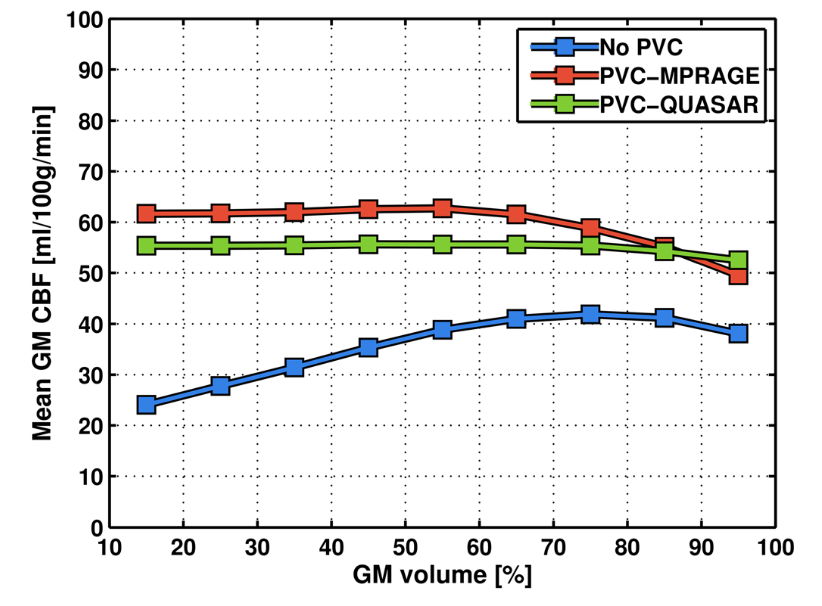
\includegraphics[width=.5\textwidth]{figures/ahlgrenplot.png}
\end{center}


\item Figure XX presents results of voxel-wise nonlinear age by sex analysis.
\end{itemize}

\section{Discussion}
\label{sec:Discussion}

We have developed a general framework for PV correction in volumetric images and demonstrated its utility for correcting CBF images that are derived from any ASL sequence. Importantly, because the PNC ASL sequence included only a single TI, we were unable to apply the partial volume correction of \citep{chappell2011partial} which requires multi-TI ASL. Particularly for imaging studies that use single TI aquisition of ASL, we believe ISLA images are a compelling option for PV correction.

Our method builds upon previous work in the area, by employing a kernel-based regression approach within local neighborhoods of voxels using estimates of gray matter density. However, ISLA images improve upon the current state-of-the-art in a few notable ways. First, unlike many established methods for PV correction, we use a 3D kernel to define the local neighborhoods. This improvement is possible due to recent advances in high performance computing, since it requires more memory and computational power than fitting local regressions within 2D image slices. Second, previous methods have relied on assumptions that are unlikely to hold in real imaging data, namely, that the effects of partial voluming are constant within local neighborhoods and that the voxels within local neighborhoods of an individual's image are independent \citep{asllani2008regression,ahlgren2014partial}. Our method accounts for non-constant effects and correlation of observations within local neighborhoods by employing weights based on distance to the center voxel. Third, our approach is agnostic to the technique used to obtain ASL and is applicable more generally to any type of volumetric functional image that imaging researcher aim to study in a group-level analysis. For example, our framework could be used in studies of local connectivity (ALFF) or regional homogeneity (REHO), and may be critical to analyses targeting developmental effects of the coupling between these functional measurements and brain structure.

\vspace{5mm}
\noindent PARAGRAPH ON LIMITATIONS:
\begin{itemize}
\item Smoothing effects. Note that \citep{chappell2011partial} talks about this as a disadvantage of other methods.
\end{itemize}


\newpage


%\begin{equation}
%SPE(v) = g\left \{ \frac{\lambda_{1}(v)}{\sum_{k=1}^{K}\lambda_{k}(v)} \right\}
%\end{equation}

%\begin{equation}
%g(x) = \frac{K}{K-1}\left\{ x - \frac{1}{K} \right\}
%\end{equation}


%\bibliographystyle{apalike}
\bibliography{cites.bib}

\end{document}